\documentclass{report}
\usepackage[utf8]{inputenc}				
\usepackage{mdframed}			
\usepackage{graphics}	
\usepackage{graphicx}
\usepackage{xspace}
\usepackage{amsmath}
\usepackage{wrapfig}
\usepackage[a4paper, total={6.5in, 9.5in}]{geometry}

\begin{document}	
\begin{titlepage} 			
\centering						
\vspace*{\fill}					
										
\huge{STANFORD UNIVERSITY}\\	
\vspace{1 cm}
\LARGE{STATS 245 Final Project}
\vspace{2 cm}
\begin{mdframed}					
\centering
\LARGE{Does Homelessness Make People Less Physically Competent?}
\end{mdframed}

\vspace{3 cm}

\begin{flushleft}
\large{Name: Anyu Zhu\\			
ID: 006402340 \\
Date: August 2019\\}

\vspace{3 cm}
\underline{Summary}\\[0.2in]
This report analyzes whether homelessness makes people less physically competent, based on certain data set. The relationship between homelessness and physical component score is evaluated using linear regression. Potential con-founders are tested to improve the accuracy of the model. Regression method and propensity scores are adopted during the process and significance of the factors included have been detailedly tested.
\vspace*{\fill}	
\end{flushleft}
\end{titlepage}						

\section{Relationship Between Factors}

\subsection{The Relationship Between Exposure(homeless) and Outcome(pcs)}
We regress the exposure "homeless" onto outcome "pcs", and get the first regression model:
\[pcs = -2.064 * homeless + 49.001\]
The p-value is 0.04216, which indicates that the relationship between homelessness and physical competence is significant. There is a negative correlation between "pcs" and "homeless". Homeless people tend to have lower physical component score. The adjusted R-squared of the model is 0.006926, which is quite small. We need to move on to explore the con-founders and adjust the model.

\subsection{Selection of Con-founders}
Apart from the exposure and outcome, there are in total fourteen factors where we should select the potential con-founders to improve the model. We adpoupt the standard that: if the changes in $\beta$ is larger than 10\% after including the factor into our regression model, we see the factor as a possible potential con-founder and move on to furtehr selection process.

\begin{center}
 \begin{tabular}{||c c c c||} 
 \hline
 Variable & $\beta_1$ - $\beta_1'$ & Ratio & larger than 10\% \\
 \hline\hline
 age & -0.4124 & 0.1998 & Yes \\ 
 \hline
 anysubstance & -1.2021 & 0.5824 & Yes \\
 \hline
 a15a & 0.2192 & -0.1062 & Yes \\
 \hline
 a15b & -1.4643 & 0.7094 & Yes \\
 \hline
 cesd & -0.5392 & 0.2613 & Yes \\
 \hline
 d1 & -0.3616 & 0.1752 & Yes \\
 \hline
 daysanysub & -1.2119 & 0.5871 & Yes \\
 \hline
 daysdrink & -1.2053 & 0.5840 & Yes \\
 \hline
 drugrisk & -0.1139 & 0.0552 & No \\
 \hline
 female & 0.3534 & -0.1712 & Yes \\
 \hline
 g1b & -0.3922 & 0.1900 & Yes \\
 \hline
 i1 & -0.9443 & 0.4575 & Yes \\
 \hline
 mcs & -0.1540 & 0.0746 & No \\
 \hline
 pss\_fr & -0.2309 & 0.1119 & Yes \\
 \hline
\end{tabular}
\end{center}
By comparing the ratio of changes in $\beta_1$, we can select out the possible potential con-founders: if the ratio is larger than 10\%, then the factor can be selected as a potential con-founder. We then move on to test whether the factors can improve the model by comparing the p-value and adjusted R-squared of the regression model after adding the factor. The following part only displays the potential con-founders which improves the regression model (significant p-value and larger adjusted R-square), the evaluation process of the rest factors will be included in appendix.
\begin{itemize}
    \item age: the regression model after including the age factor: The p-value is reduced to 1.412e-06 and adjusted R-squared increased to 0.0539.\[pcs = -1.6515 * homeless - 0.31074 * age + 59.88949\] 
    \item a15b: the regression model after considering number of nights on streets: the p-value is reduced to 2.039e-08 and adjusted R-squared increased to 0.0763. \[pcs = -0.3056 * homeless - 0.2986 * age - 0.0652 * a15b + 59.4655\]
    \item cesd: after adding depression scale to the improved model above: the p-value is decreased to 3.888e-15 and adjusted R-squared increased to 0.1437. \[pcs = -0.1990 * homeless - 0.3019 * age - 0.0461 * a15b - 0.2304 * cesd + 66.9135\]
    \item d1: the times hospitalized for medical problems is also counted as a con-founder, the p-value is decreased to less than 2.2e-16 and adjusted R-squared is 0.1787 now.
    \begin{align*}
        pcs = &- 0.0817 * homeless - 0.2598 * age - 0.0423 * a15b - 0.2172 * cesd\\
              & - 0.3396 * d1 + 65.9327
    \end{align*}
    \item female: the regression model after considering the gender: The p-value is less than 2.2e-16 and adjusted R-squared increased to 0.1865.
    \begin{align*}
        pcs = &- 0.3484 * homeless - 0.2531 * age - 0.0420 * a15b - 0.2011 * cesd\\
              & - 0.3359 * d1 - 2.5465 * female + 65.8722
    \end{align*}
    \item g1b: The next con-founder which can improve the regression model is thoughts of suicide, the p-value is less than 2.2e-16 and adjusted R-squared increased to 0.1875.
    \begin{align*}
        pcs = &-0.1586 * homeless - 0.2590 * age - 0.0440 * a15b - 0.1855 * cesd\\
              & - 0.3325 * d1 - 2.3870 * female - 1.3638 * g1b + 65.8371
    \end{align*}
    \item i1: The next con-founder we need to consider is the daily consumption of drinks: p-value is significantly small and adjusted R-squared increased to 0.1879.
    \begin{align*}
        pcs = &-0.0301 * homeless - 0.2472 * age - 0.0405 * a15b - 0.1806 * cesd - 0.3158 * d1\\
              & - 2.5434 * female - 1.2646 * g1b - 0.0282 * i1 + 65.6235
    \end{align*}
\end{itemize}
In all, after all evaluation process, we selected seven con-founders in total: age, number of nights on street (a15b), depression scale (cesd), times hospitalized for medical situation (d1), gender (female), thoughts of suicide (g1b), and daily drinks consumption (i1).

\subsection{Relationship Between Con-founders and Exposure}
We then evaluate the relationship between con-founders and exposure. Since exposure: homeless has binary values, for binary factors (gender, thoughts of suicide), we compare the number of homeless people in different categories; for factors which have continuous value, we adopt logistic regression and compare the coefficient of the factor in the regression model. The following are the results:\\[0.1in]
Binary con-founders:
\begin{center}
 \begin{tabular}{||c | c c | c || c c | c ||} 
 \hline
 Factors & male & female & $\chi^2$ and p-value & not suicide & suicide & $\chi^2$ and p-value\\ 
 \hline
 not homeless & 177 & 67 & 129.6 & 189 & 55 & 100.63 \\
 
 homeless & 169 & 40 & $<$ 2.2e-16 & 137 & 72 & $<$ 2.2e-16 \\
 \hline
\end{tabular}
\end{center}
From the table, we can see that: The chi-square test shows the significance in differences between frequencies. Although male takes up a much larger proportion of sample size, the proportion of homeless among male is also larger than that of female. Number of people who had thoughts of suicide is smaller in sample, among these people who had negative thoughts, homeless people takes a larger proportion. We then draw to the conclusion that negative thoughts and homelessness has positive correlation, and gender also has a significant effect on exposure. \\[0.1in]
Continuous Con-founders:
\begin{center}
 \begin{tabular}{|| c | c | c | c | c ||} 
 \hline
 Con-founder & age & cesd & d1 & i1 \\ 
 \hline
 Coefficient & 0.0224 & 0.0141 & 0.0253 & 0.0271 \\
 \hline
 p-value & 0.0685 & 0.0647 & 0.1921 & 1.71e-6 \\
 \hline
\end{tabular}
\end{center}
Based on the coefficients generated from logistic regression, we can see that these four con-founders may potentially cause homelessness. From the p-values, we can see that except for "times hospitalized for health problems" (d1) is much less significant than others, number of drinks is a important driving factor of homelessness, and cesd, age also has effect. In further process, we will consider whether d1 is an appropirate con-founder.\\
* A special factor "a15b" fails to run the logistic regression, we count the population of homeless people in different range of "nights on street": 53.86\% of sample (244 people) have 0 nights on street and is not homeless, the rest are all homeless and spend different numbers of nights on street. Thus, "a15b" has a positive correlation with homelessness.

\subsection{Relationship Between Con-founders and Outcome}
The following is the evaluation of the relationship between con-founders and outcome: physical component score. Since physical competence is of continuous values, we calculate the correlation between pcs and con-founders (except gender and thoughts of suicide, which are binary con-founders). \\[0.1in]
Continuous con-founders: 
\begin{center}
 \begin{tabular}{||c c c c c c||} 
 \hline
 cor & age & a15b & cesd & d1 & i1  \\ 
 \hline\hline
 pcs & -0.2287 & -0.1915 & -0.2927 & -0.2576 & -0.1963\\
 \hline
\end{tabular}
\end{center}
From the correlation coefficients, the above con-founders have negative correlation with physical component score: older people tend to have lower physical competence; increasing number of nights on street cause slightly decrease in physical competence; higher depression scale does harm to physical competence; number of hospitalized indicates weaker physical competence, and drinking decrease the physical competence score. \\[0.1in]
Binary con-founders: We calculate the average physical component score within each category. 
\begin{center}
 \begin{tabular}{||c | c c || c c ||} 
 \hline
 mean & female & male & not suicide & suicide \\ 
 \hline
 pcs & 45.0164 & 48.9862 & 49.0408 & 45.5014 \\
 \hline
\end{tabular}
\end{center}
By the average values, we can draw to the conclusion that male tend to have higher physical competence; People who never experienced negative thoughts related to suicide have higher physical component scores. 

\section{Casual Inference and Improved Model}
After basic selection process of potential con-founders, our current model is:  
\begin{align*}
pcs = &-0.0301 * homeless - 0.2472 * age - 0.0405 * a15b - 0.1806 * cesd - 0.3158 * d1\\
& - 2.5434 * female - 1.2646 * g1b - 0.0282 * i1 + 65.6235
\end{align*}
To further increase the accuracy of the model, we use propensity scores to test the validity of all the factors included in the model. Since the number of con-founders is quite large, we use propensity score measure the sample and the con-founders.\\
\begin{itemize}
    \item Test for age:\\
    \begin{minipage}{0.5\linewidth}
         From the histogram generated from the propensity scores, we can see there is reasonable amount of overlapping between homeless and non-homeless group, so we keep age as an effective con-founder.
    \end{minipage}
    \begin{minipage}{0.5\linewidth}
        \centering
        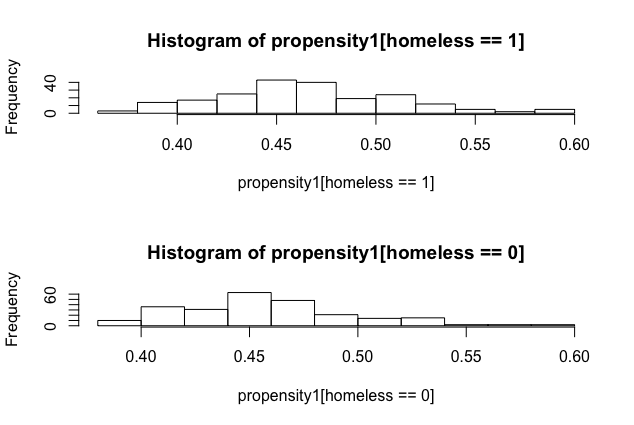
\includegraphics[scale=0.25]{1.jpg}
    \end{minipage}
    \item Test for a15b:\\
    \begin{minipage}{0.5\linewidth}
         From the histogram generated from the propensity scores, the amount of overlapping areas is small, indicating a lack of good balance. Thus we remove "a15b" from con-founders. Possible reason: number of nights on streets is so hlghly related to the factor "homeless" itself.
    \end{minipage}
    \begin{minipage}{0.5\linewidth}
        \centering
        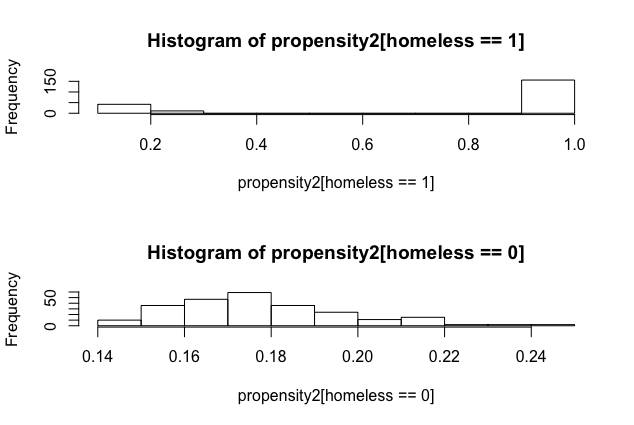
\includegraphics[scale=0.25]{2.png}
    \end{minipage}
    \item Test for cesd:\\
    \begin{minipage}{0.5\linewidth}
         From the histogram of propensity scores of age and cesd, we can see a significant amount of overlap between homeless and non-homeless, indicating that cesd also has similar effect on both homeless and non-homeless. So we keep it as a con-founder.
    \end{minipage}
    \begin{minipage}{0.5\linewidth}
        \centering
        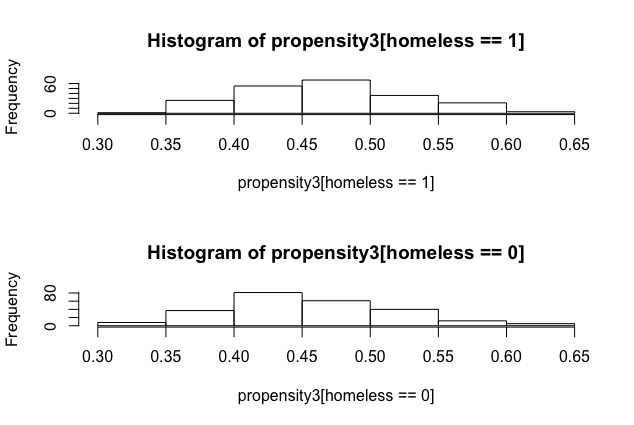
\includegraphics[scale=0.25]{3.png}
    \end{minipage}
    \item Test for d1:\\
    \begin{minipage}{0.5\linewidth}
         From the histogram of propensity scores including d1, we can see that the area of overlapping decreased significantly. Thus we remove d1 from con-founders. Possible reason: times of hospitalized for medical problems strongly indicates the level of pcs, and is highly related with other factors.
    \end{minipage}
    \begin{minipage}{0.5\linewidth}
        \centering
        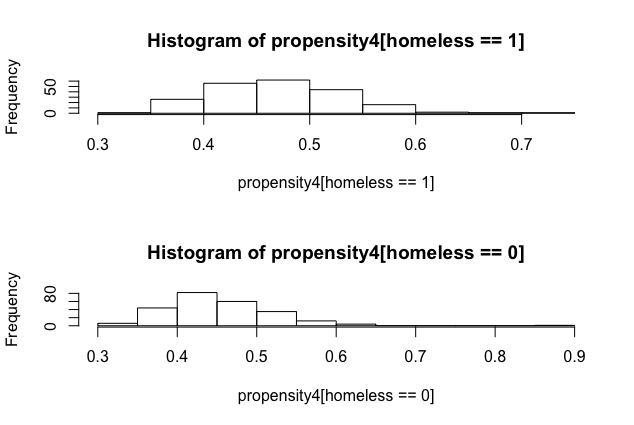
\includegraphics[scale=0.25]{4.png}
    \end{minipage}
    \item Test for gender:\\
    \begin{minipage}{0.5\linewidth}
         From the histogram of the propensity scores of model including gender, we can see the propensity scores for both homeless group and non-homeless group overlap well. This indicates that gender affect both groups at similar level. So we keep it as an effective con-founder. 
    \end{minipage}
    \begin{minipage}{0.5\linewidth}
        \centering
        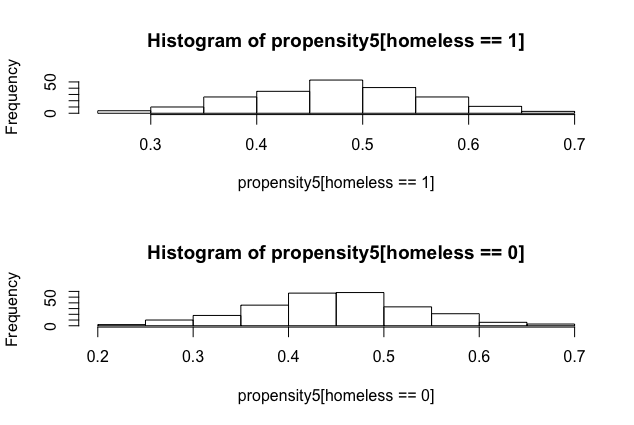
\includegraphics[scale=0.25]{5.png}
    \end{minipage}
    \item Test for g1b:\\
    \begin{minipage}{0.5\linewidth}
         From the histogram of the propensity scores of model including "g1b", we can see that the area of overlapping is significant, indicating the similarity of two sample groups. Thus we include g1b as a significant con-founder. 
    \end{minipage}
    \begin{minipage}{0.5\linewidth}
        \centering
        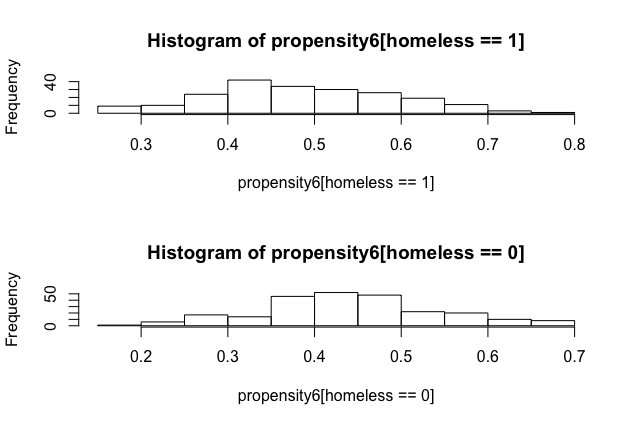
\includegraphics[scale=0.25]{6.png}
    \end{minipage}
    \item Test for i1:\\
    \begin{minipage}{0.5\linewidth}
        From the histogram of propensity scores of model including "i1", we can observe a significant overlap of two groups. Data won't extrapolate outside the range when we adjust Thus we keep i1 as an effective con-founder.  
    \end{minipage}
    \begin{minipage}{0.5\linewidth}
        \centering
        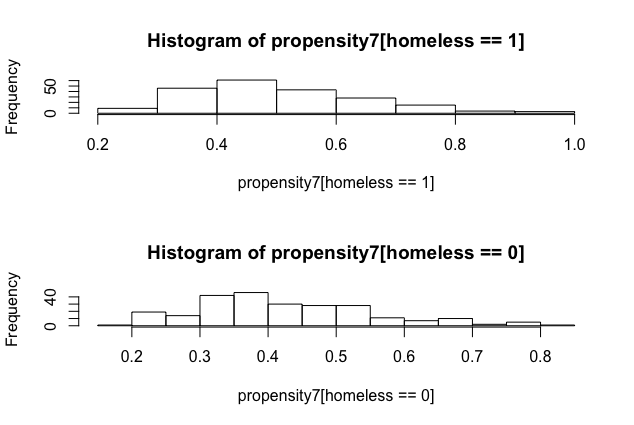
\includegraphics[scale=0.25]{8.png}
    \end{minipage}
\end{itemize}
After going through all the con-founders and going through the histograms, we include the propensity score as a continuous covariate in the regression model. Our regression model looks like the following:
\[pcs = -0.8608 * homeless - 14.8605 * propensity + 55.3018\]
The p-value is 3.559e-05, which is far less than 0.05, indicating the significance of the model. From the histogram of propensity scores above, we can see that there is a good matching between homeless group and non-homeless group. The coefficient of homeless in this model is negative, which means being homeless has negative effect on physical competence. 
\section{Conclusion}
After all the analysis process, to answer the question: Does homelessness makes people less physical competent? We can draw to the conclusion that with a negative coefficient of the factor "homeless", being homeless has negative effect on people's physical competence. However, we cannot judge their relationship by simply conducting regression between homelessness and people's physical component scores. Some other factors also plays important roles: age; depression scale; gender; thoughts of getting suicide; number of daily drinks. Through doing regression, calculating correlations, and comparing propensity scores, we find these factors has significant on both the exposure(homeless) and the outcome(physical competence), they all exert similar effect on both the homeless group and non-homeless groups. From our final model with propensity, we can see that apart from the factor "homeless" itself, these factors in total actually decrease people's physical competence significantly. 
\newpage
\section{Appendix}
\subsection{Code}
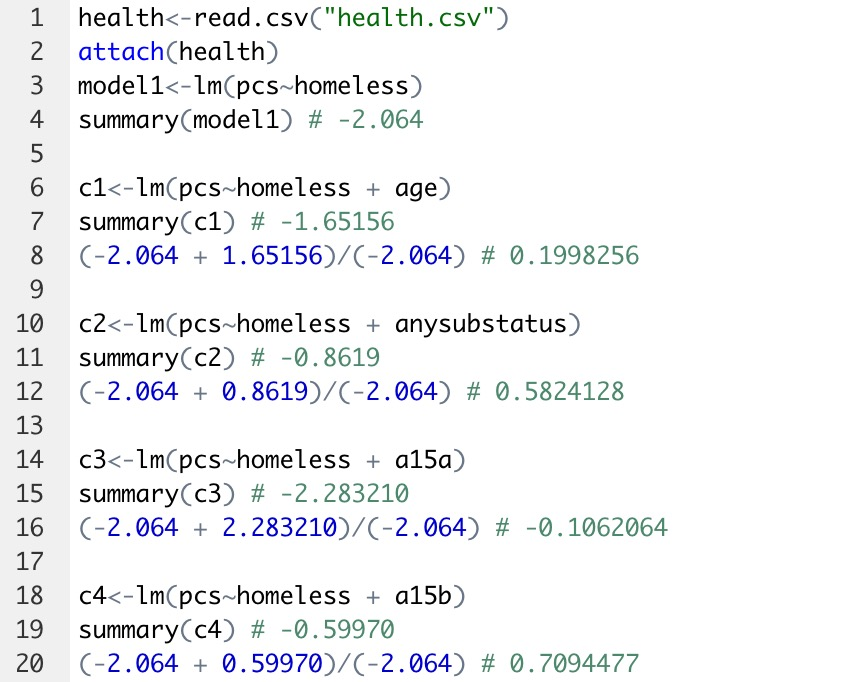
\includegraphics[scale=0.3]{a.jpeg}\\
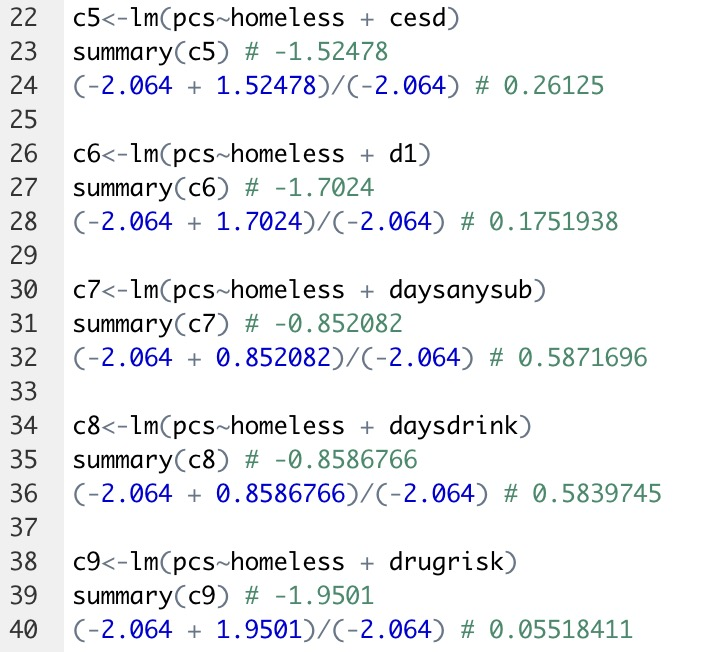
\includegraphics[scale=0.3]{b.jpeg}\\
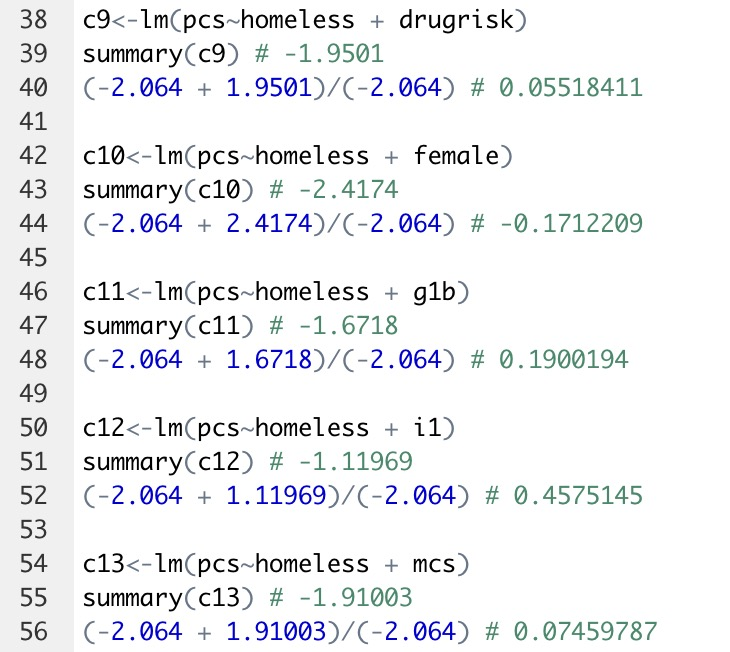
\includegraphics[scale=0.3]{c.jpeg}\\
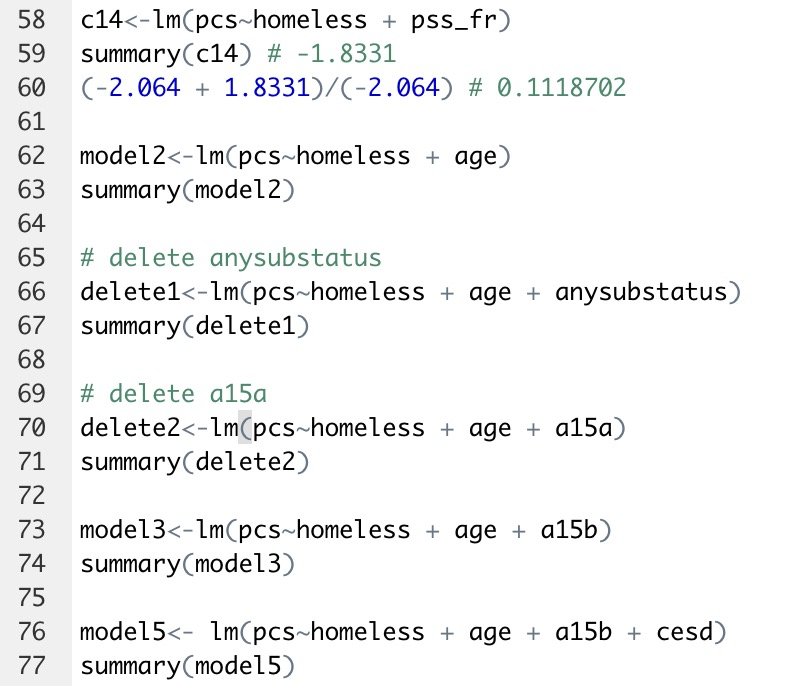
\includegraphics[scale=0.3]{d.jpeg}\\
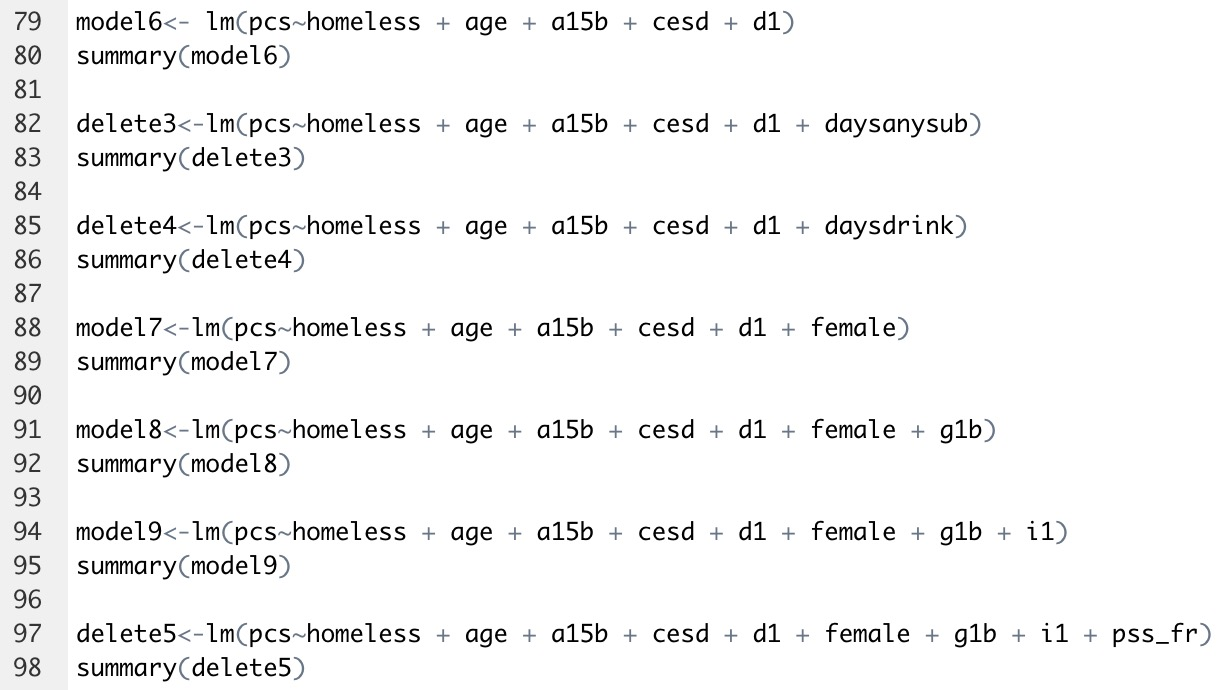
\includegraphics[scale=0.3]{e.jpeg}\\
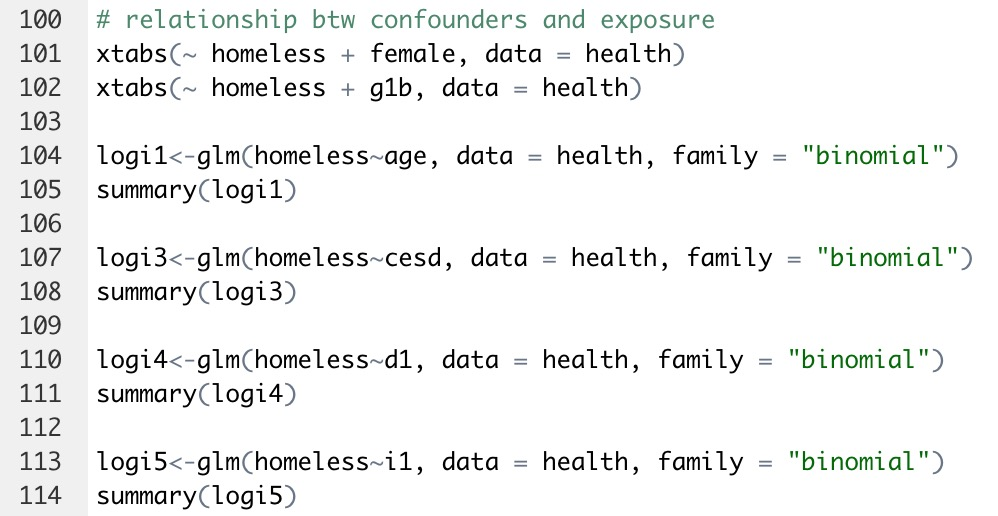
\includegraphics[scale=0.3]{f.jpeg}\\
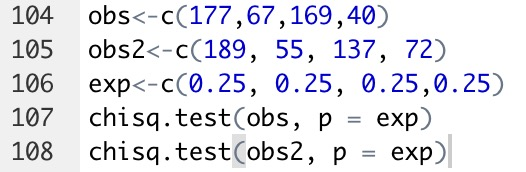
\includegraphics[scale=0.3]{6.jpeg}\\
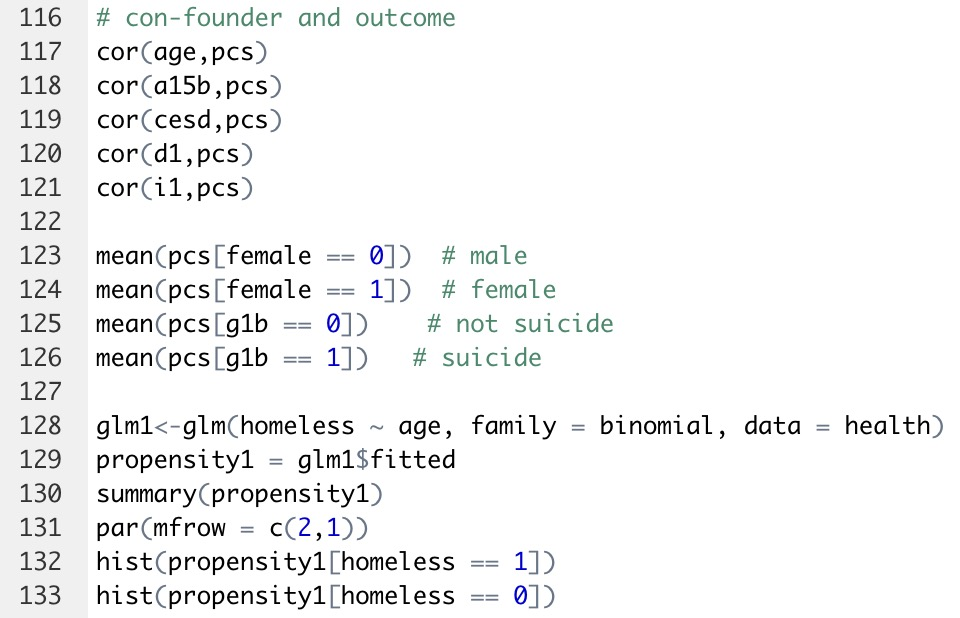
\includegraphics[scale=0.3]{g.jpeg}\\
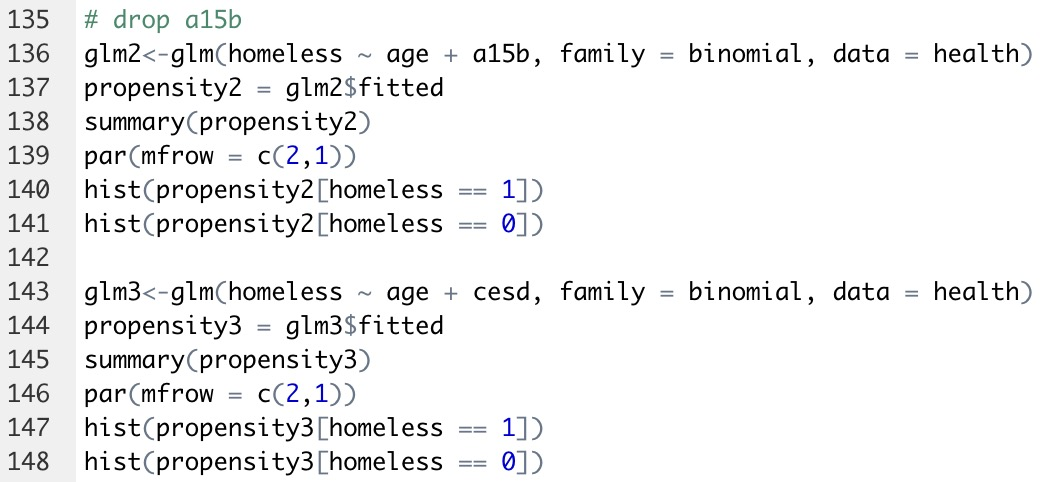
\includegraphics[scale=0.3]{h.jpeg}\\
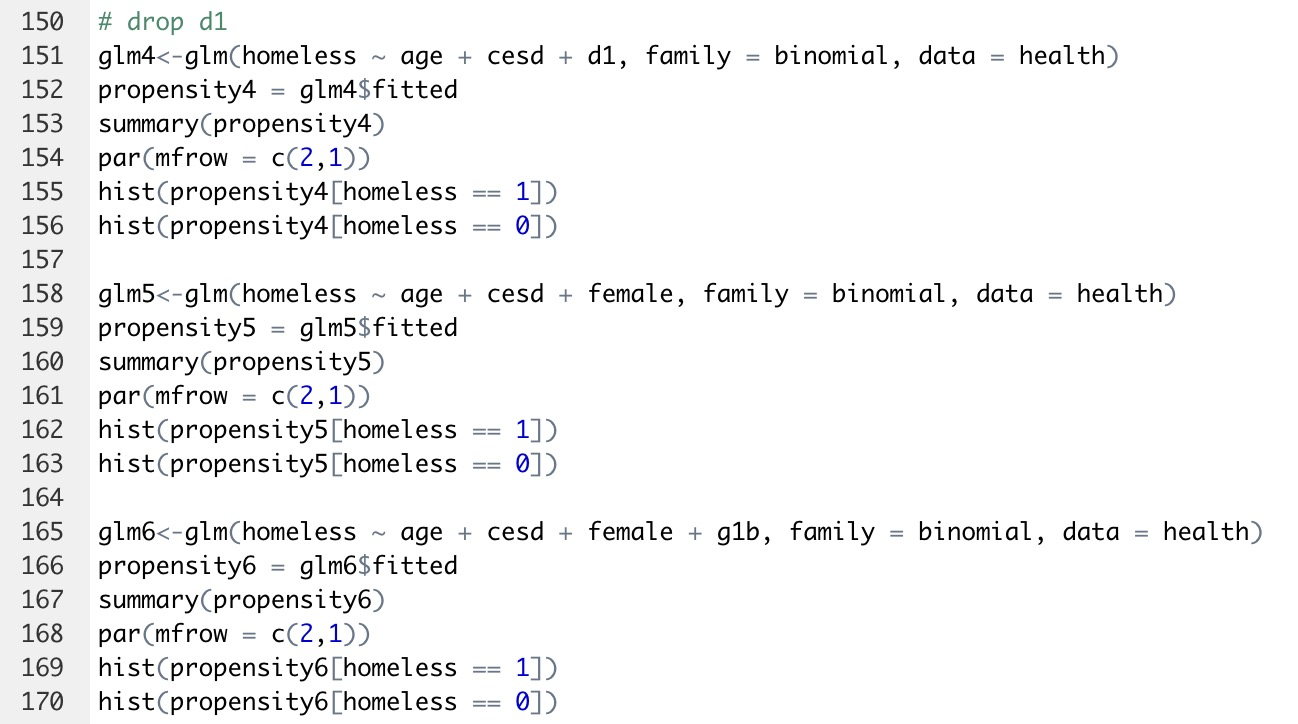
\includegraphics[scale=0.3]{i.jpeg}\\
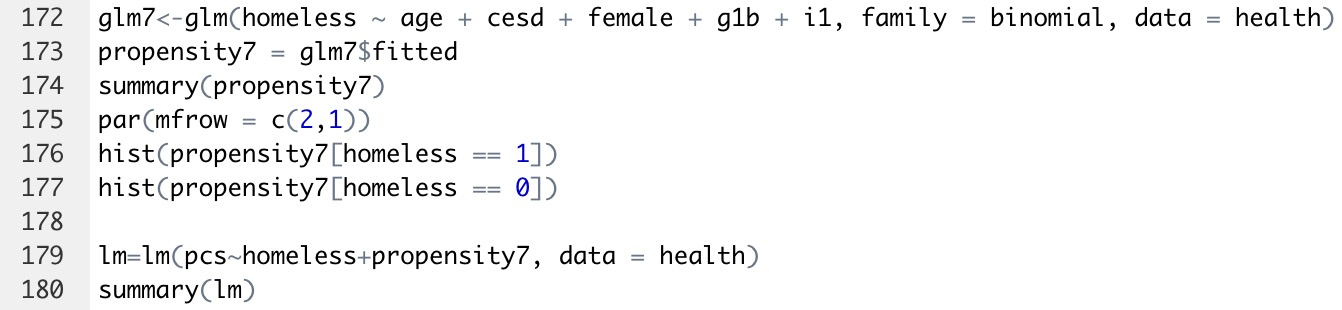
\includegraphics[scale=0.3]{j.jpeg}
\subsection{Additional selection process of con-founders}
\begin{itemize}
    \item After including "anysubstatus": p-value: 0.003393; Adjusted R-squared: 0.04309. p-value increased while adjusted R-squared decreased compared with the model including only age. So we do not take it as a con-founder.
    \item After including "a15a": p-value: 4.654e-06; Adjusted R-squared:  0.05303. p-value increased while adjusted R-squared decreased compared with that only includes age. So we do not consider it as a con-founder.
    \item After including "daysanysub": p-value: 8.36e-11; Adjusted R-squared: 0.1979. p-value increased and adjusted R-squared decreased compared with the model after including "d1". So we drop this factor.
    \item After including "pss\_fr": Adjusted R-squared: 0.187, a little bit smaller than that of the model after including "i1", which means less accuracy of the model. So we drop "pss\_fr".
\end{itemize}
\end{document}	
